\documentclass[conference]{IEEEtran}
\usepackage{cite}
\usepackage{amsmath,amssymb,amsfonts}
\usepackage{algorithmic}
\usepackage{graphicx}
\usepackage{textcomp}
\usepackage{xcolor}
\usepackage{float}
\usepackage{caption}


\graphicspath{{./img2/}{./images/25_50/}{./images/1_25/}}
\begin{document}
\title{COMP90086 Computer Vision Final Project\\
Stereo Disparity
}
\author{
\IEEEauthorblockN{Jun Li Chen}
\IEEEauthorblockA{1043258}
\and
\IEEEauthorblockN{Tianli Cheng}
\IEEEauthorblockA{1128434}
}
\maketitle
\section{Introduction}
\section{Methodology}
\section{Evaluation}
\begin{figure}[H]
    \centering
    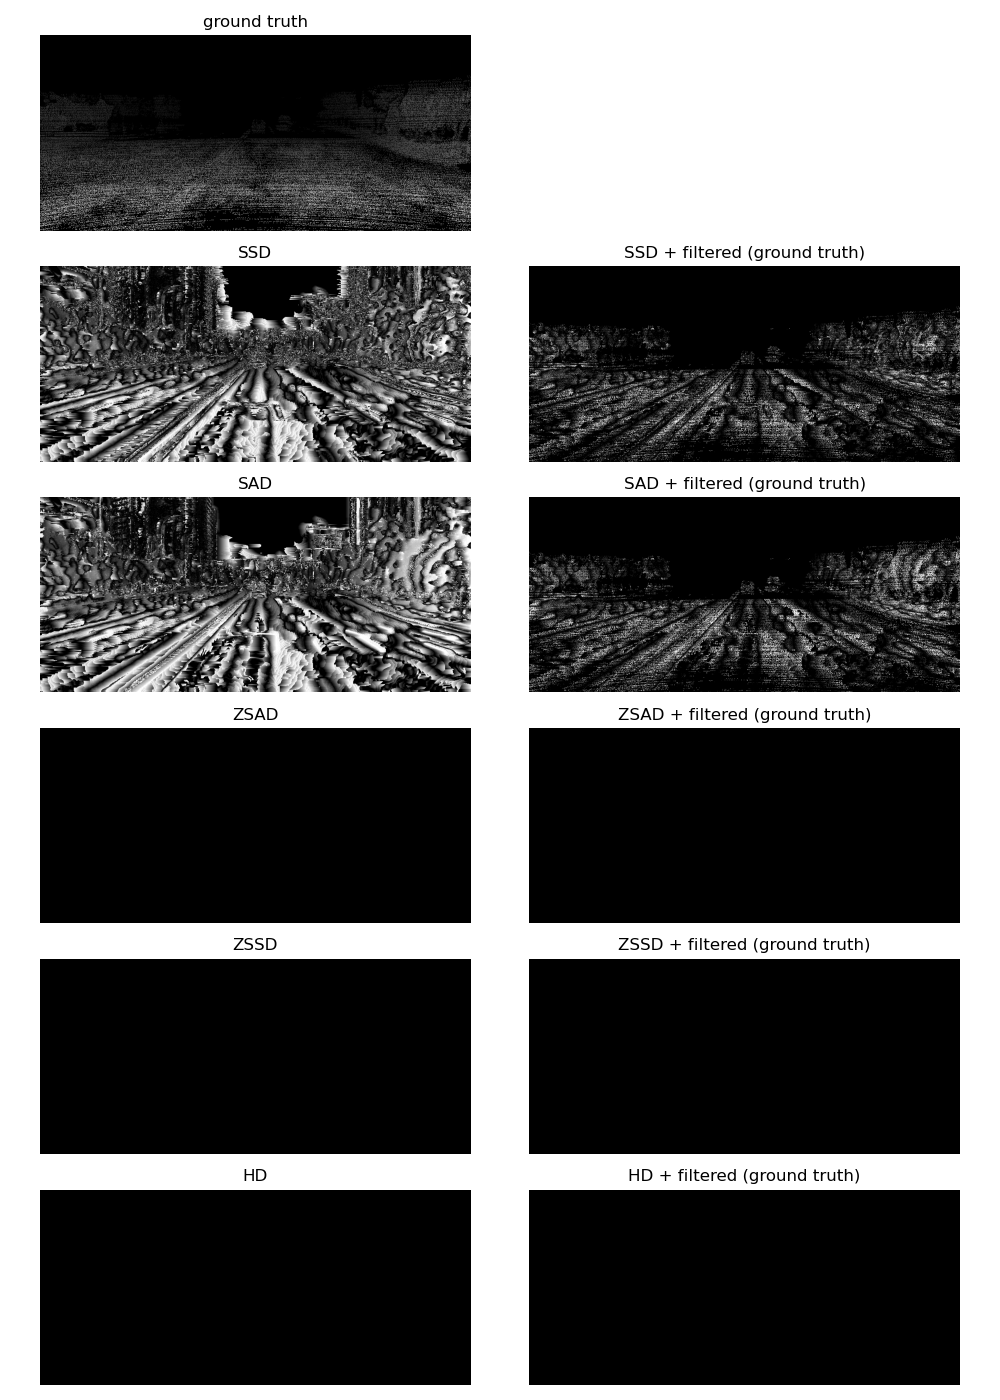
\includegraphics[width=8.8cm]{702_output_1_25.png}
    \captionof{figure}{Disparity map output with block size 1 \& search size 25.}
\end{figure}
\begin{figure}[H]
    \centering
    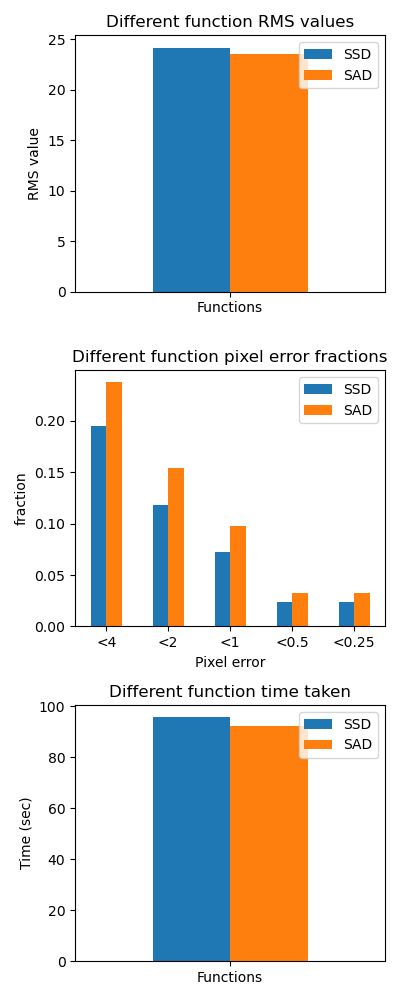
\includegraphics[height=11cm]{702_stats_1_25.png}
    \captionof{figure}{Disparity performance with block size 1 \& search size 25. (See Appendix A for bar chart values)}
\end{figure}
\section{Improvements}
In digital image processing, different similarity measurement functions exist including the sum of absolute difference (SAD), the sum of square difference (SSD), etc. Six functions have been chosen among these to make a performance comparison in this report. They are SAD, SSD, the zero-mean sum of absolute difference (ZSAD), the zero-mean sum of square difference (ZSSD), and hamming distance of census transform (HDCT). 

SAD of block W1 and block W2 was calculated by summing up the intensity differences between each corresponding pixel pair, as in:
\begin{equation*}
    SAD=\sum^{n}_{i=0}\sum^{m}_{j=0}|W1[i,j]-W2[i,j]|
\end{equation*}

Similarly, the SSD of block W1 and block W2 was calculated by summing up the square of intensity differences between each corresponding pixel pair, as in:
\begin{equation*}
    SSD=\sum^{n}_{i=0}\sum^{m}_{j=0}(W1[i,j]-W2[i,j])^2
\end{equation*}

SSD is more discriminative compared to SAD since the differences between image patches are amplified by squaring [1]. It means that SSD is more sensitive to large differences compared to SAD. In case there is one single pixel holding a value that is much larger than the corresponding pixel in the other image block compared to the rest, the dissimilarity score given by SSD can be much higher than what will be given by SAD. It means that those pixels holding small differences are more likely to be ignored by SSD.

Hence, two other similarity measurement functions, ZSAD and ZSSD, are chosen to perform a certain degree of normalization avoiding the result being biased by large values. ZSAD between blocks is calculated by summing up the deviation differences between each corresponding pixel pair, as in:

\begin{equation*}
    \begin{aligned}
        ZSAD= {} & \sum^{n}_{i=0}\sum^{m}_{j=0}|(W1_{[i,j]}-\frac{1}{nm}\sum^{n}_{i=0}\sum^{m}_{j=0}W1_{[i,j]})\\
        & -(W2_{[i,j]}-\frac{1}{nm}W2_{[i,j]})|
    \end{aligned}
\end{equation*}

It first finds the differences between each element and the mean intensity value in both image blocks, then finds the absolute differences of the corresponding deviation. Similarly, ZSSD was calculated by summing up the square of deviation differences between each corresponding pixel pair, as in:
\begin{equation*}
    \begin{aligned}
        ZSSD= {} & \sum^{n}_{i=0}\sum^{m}_{j=0}((W1_{[i,j]}-\frac{1}{nm}\sum^{n}_{i=0}\sum^{m}_{j=0}W1_{[i,j]})- \\
        & (W2_{[i,j]}-\frac{1}{nm}W2_{[i,j]}))^2
    \end{aligned}
\end{equation*}

By only keeping the deviation, these functions are less sensitive to a general shift in intensity which can be caused by a change in lightning. However, normalization can be taken further by including the relation of a single pixel with the image block it belongs to into consideration. Normalized Cross-Correlation (NCC) is one of the most classic metrics including local relations when mapping similarity between images. It sums the cross-correlation between blocks and then divides it by the product of the square root of the sum of the square of both image blocks, as in:

\begin{equation*}
    NCC=\frac{\sum^{n}_{i=0}\sum^{m}_{j=0}W1_{[i,j]}*W2_{[i,j]}}{\sqrt{\sum^{n}_{i=0}\sum^{m}_{j=0}W1_{[i,j]}^2}*\sqrt{\sum^{n}_{i=0}\sum^{m}_{j=0}W2_{[i,j]}^2}}
\end{equation*}

NCC is less sensitive to a linear change in lightning intensity but computationally expensive [3]. Different approaches, such as coarse-to-fine and multi-resolution search, exist to reduce the computational complexity for NCC, but these include much more complex methods like neural networks beyond the scope of this report. Hence, HDCT has been selected as an alternative to NCC and also normalized the image pattern by local correlation. 

The census transform records each pixel holding a lower intensity compared to the center pixel as 0 and the rest as 1. Figure 1 gives an example of how census transform works in a 3 by 3 window.

\begin{figure}[H]
    \centering
    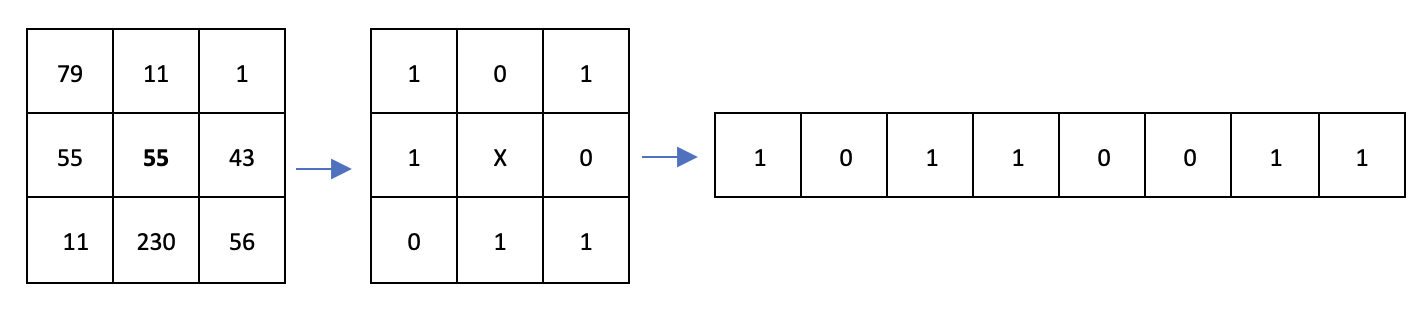
\includegraphics[width=8cm]{fig1.png}
    \caption{Census transform}
\end{figure}

It represents each pixel's relation to the center pixel in a binary form. Therefore, it is non-parametric and insensitive to radiometric variations [2].

The Hamming distance of the census transform between two blocks is calculated by performing a XOR operation on the two 1-D binary representations. By counting the number of 1 existing in the outcome of XOR between blocks, the result represents the number of different patterns. Figure 2 gives an example of how it works.

\begin{figure}[H]
    \centering
    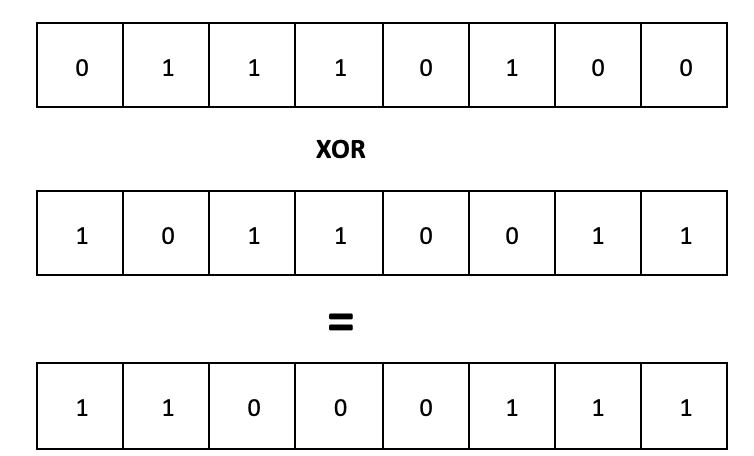
\includegraphics[width=6cm]{fig2.png}
    \caption{Hamming distance of Census transform}
\end{figure}

It is found that the computational time of pixel-wise disparity calculation is extremely long in this case since experiment photos all have 400 by 881 pixels. The function will iterate $400*881*88=31011200$ times if it searches every pixel on the left image and finds correspondence on the right image on the same line. The iteration must be deducted to improve the method's feasibility.

By setting a search size, the program will not iterate over all pixels laying on the same line on the right image but only within a defined searching window of fixed size. Meanwhile, the function will search those image blocks with center coordinates closer to the original coordinate of the block cropped from the left image first, since the correspondence is more likely to be found in those locations.

The number of iterations is further deducted by assuming each pixel in the image block holds the same disparity. By replacing pixel-wise correspondence searching with block-wise correspondence searching, the maximum number of iterations becomes:
\begin{equation*}
    \frac{400*881}{block\_width*block\_height*window\_size}
\end{equation*}

\section{Comparison / Conclusion}
asdf
\begin{figure}[H]
    \centering
    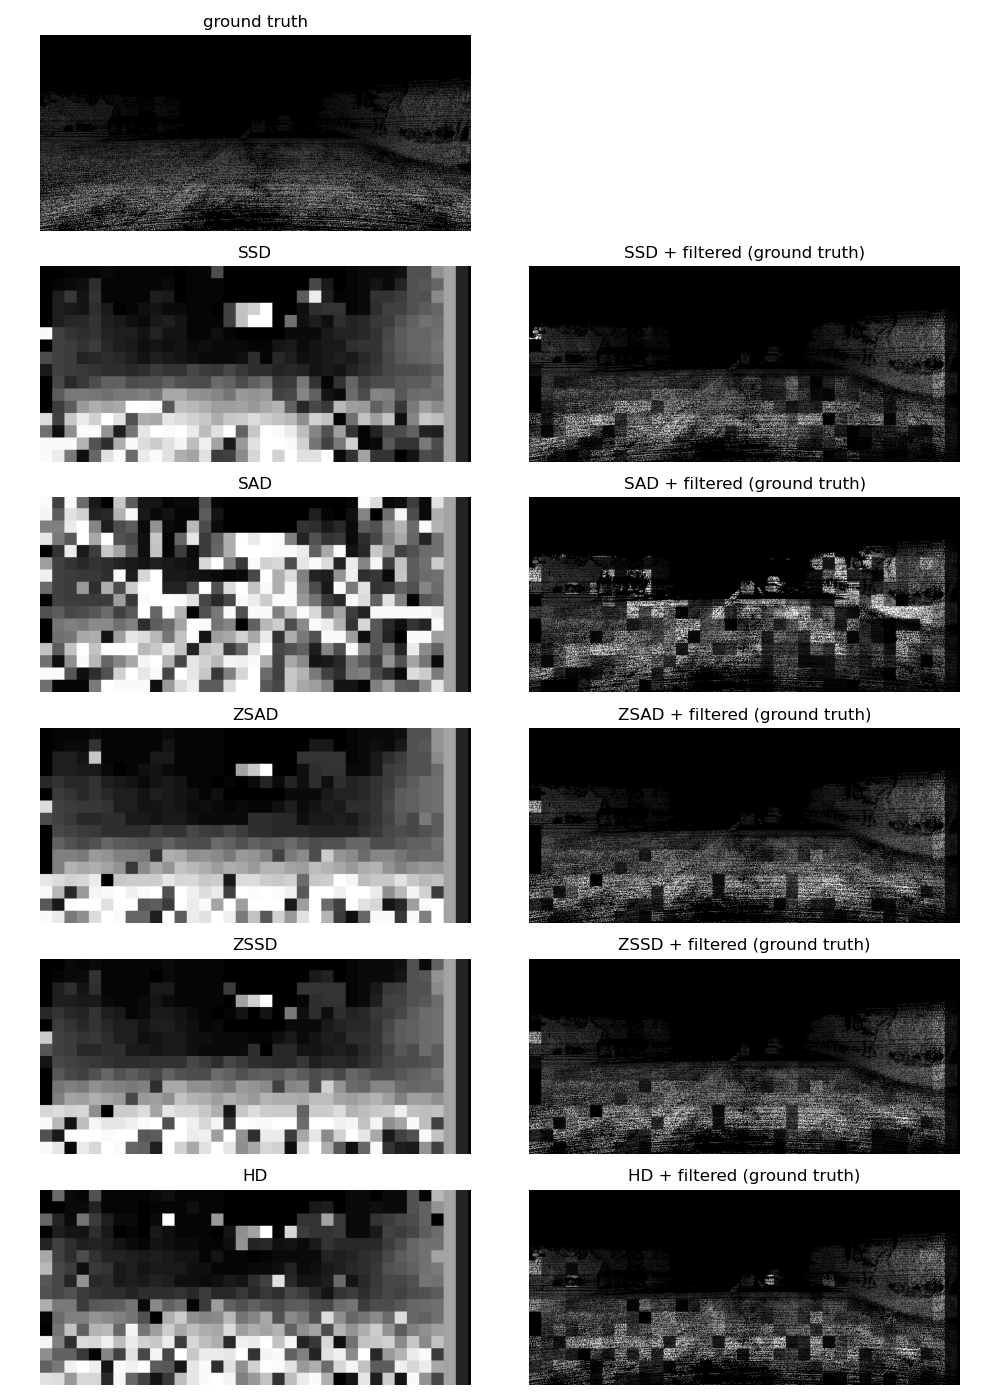
\includegraphics[width=8.8cm]{702_output_25_50.png}
    \captionof{figure}{Disparity map output with block size 25 \& search size 50.}
\end{figure}
\begin{figure}[H]
    \centering
    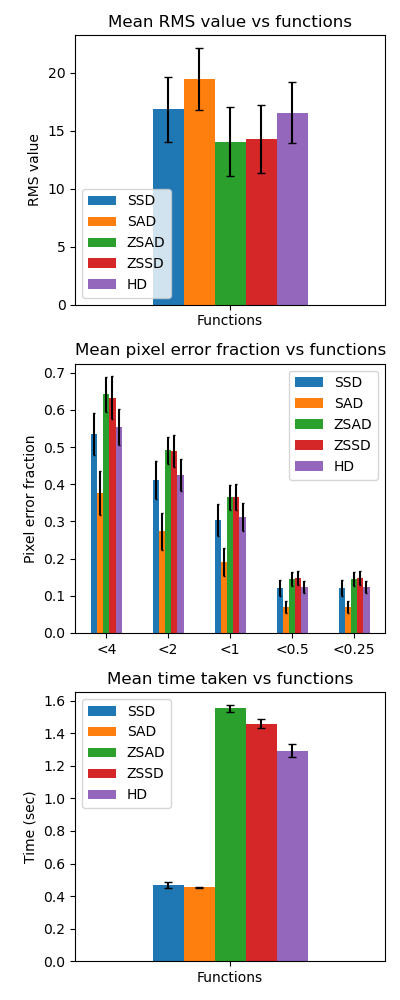
\includegraphics[height=11cm]{stats_25_50.png}
    \captionof{figure}{Disparity performance with block size 25 \& search size 50. (See Appendix A for bar chart values)}
\end{figure}

\newpage
\begin{thebibliography}{00}
\bibitem{1} Schmidt, A., Kraft, M. and Kasiński, A., 2010. An Evaluation of Image Feature Detectors and Descriptors for Robot Navigation. Computer Vision and Graphics, pp.251-259.
\bibitem{2} Sarika, S., Deepambika, V. and Rahman, M., 2015. Census Filtering Based Stereomatching under Varying Radiometric Conditions. Procedia Computer Science, 58, pp.315-320.
\bibitem{3} Tsai, D. and Lin, C., 2003. Fast normalized cross correlation for defect detection. Pattern Recognition Letters, 24(15), pp.2625-2631.
\end{thebibliography}
\vspace{12pt}

\section*{Appendix A}
\begin{center}
    \begin{tabular}{l c c c c c}
        \textbf{Function} & \textbf{SSD} & \textbf{SAD} & \textbf{ZSAD} & \textbf{ZSSD} & \textbf{HD} \\ [0.5ex] 
        Mean & 16.85 & 19.45 & 14.06 & 14.29 & 16.53 \\
        SD & 2.79 & 2.66 & 2.99 & 2.91 & 2.62
    \end{tabular}
    \captionof{table}{RMS statistic table values}
\end{center}
\begin{center}
    \begin{tabular}{l c c c c c}
        \textbf{Function} & \textbf{SSD} & \textbf{SAD} & \textbf{ZSAD} & \textbf{ZSSD} & \textbf{HD} \\ [0.5ex] 
        Mean ($<4$) & 0.536 & 0.376 & 0.642 & 0.634 & 0.555 \\
        Mean ($<2$) & 0.411 & 0.273 & 0.491 & 0.490 & 0.425 \\
        Mean ($<1$) & 0.303 & 0.192 & 0.365 & 0.366 & 0.313 \\
        Mean ($<0.5$) & 0.120 & 0.071 & 0.145 & 0.148 & 0.123 \\
        Mean ($<0.25$) & 0.120 & 0.071 & 0.145 & 0.148 & 0.123 \\
        & & & & & \\
        SD ($<4$) & 0.057 & 0.057 & 0.046 & 0.057 & 0.049 \\
        SD ($<2$) & 0.050 & 0.050 & 0.036 & 0.042 & 0.042 \\
        SD ($<1$) & 0.043 & 0.038 & 0.033 &  0.035 & 0.037 \\
        SD ($<0.5$) & 0.022 & 0.016 & 0.018 & 0.019 & 0.016 \\
        SD ($<0.25$) & 0.022 & 0.016 & 0.018 & 0.019 & 0.016 \\
    \end{tabular}
    \captionof{table}{Pixel error fraction statistic table values}
\end{center}
\begin{center}
    \begin{tabular}{l c c c c c}
        \textbf{Function} & \textbf{SSD} & \textbf{SAD} & \textbf{ZSAD} & \textbf{ZSSD} & \textbf{HD} \\ [0.5ex] 
        Mean & 0.466 & 0.453 & 1.553 & 1.460 & 1.294 \\
        SD & 0.019 & 0.004 & 0.022 & 0.028 & 0.042
    \end{tabular}
    \captionof{table}{Time taken statistic table values}
\end{center}

\end{document}
